\documentclass[12pt, letterpaper]{article}

\usepackage[utf8]{inputenc}
\usepackage[framemethod=TikZ]{mdframed}
\usepackage[hidelinks]{hyperref}
\usepackage{mathtools, amssymb, amsmath, cleveref, fancyhdr, geometry, tcolorbox, graphicx, float, subfigure, arydshln, url, setspace, framed, pifont, physics, ntheorem, cancel, mathrsfs}


%%% for coding %%%
\usepackage{listings}
\usepackage[ruled, vlined, linesnumbered]{algorithm2e}
\SetKwComment{Comment}{/* }{ */}
\newcommand\mycommfont[1]{\small\ttfamily\textcolor{mygreen}{#1}}
\SetCommentSty{mycommfont}

\geometry{letterpaper, left=2cm, right=2cm, bottom=2cm, top=2cm}

\pagestyle{fancy}
\fancyhead{}
\fancyhead[L]{\leftmark}
\fancyhead[R]{\rightmark}
\fancyfoot{}
\fancyfoot[C]{\thepage}
%\rfoot{\footnotesize  Tianqi Zhang}


%\renewcommand{\headrulewidth}{0pt}
\renewcommand{\footrulewidth}{0pt}

\hypersetup{
	colorlinks = true,
	bookmarks = true,
	bookmarksnumbered = true,
	pdfborder = 001,
	linkcolor = blue
}

\definecolor{emoryblue}{RGB}{1, 33, 105} 
\definecolor{lightblue}{RGB}{0, 125, 186}
\definecolor{mediumblue}{RGB}{ 0, 51, 160}
\definecolor{darkblue}{RGB}{12, 35, 64}
\definecolor{red}{RGB}{185, 58, 38}
\definecolor{green}{RGB}{72, 127, 132}
\definecolor{gray1}{RGB}{217, 217, 214}
\definecolor{gray5}{RGB}{177, 179, 179}
\definecolor{gray3}{RGB}{208, 208, 206}

\definecolor{grey}{rgb}{0.49,0.38,0.29}
\definecolor{mygreen}{rgb}{0,0.6,0}
\definecolor{grey}{rgb}{0.49,0.38,0.29}
\definecolor{mygreen}{rgb}{0,0.6,0}


%%% for coding %%%
\lstset{basicstyle = \ttfamily\small,commentstyle = \color{mygreen}\textit, deletekeywords = {...}, escapeinside = {\%*}{*)}, frame = single, framesep = 0.5em, keywordstyle = \bfseries\color{blue}, morekeywords = {*}, emph = {self}, emphstyle=\bfseries\color{red}, numbers = left, numbersep = 1.5em, numberstyle = \ttfamily\small\color{grey},  rulecolor = \color{black}, showstringspaces = false, stringstyle = \ttfamily\color{purple}, tabsize = 4, columns = flexible}


\newcounter{index}[subsection]
\setcounter{index}{0}
\newenvironment*{df}[1]{\noindent\textbf{Definition \thesubsection.\stepcounter{index}\theindex\ (#1).}}{\\}

%\newenvironment*{eg}[1]{\begin{framed}\\\noindent\textbf{Example \thesubsection.\stepcounter{index}\theindex\ #1}\\ }{\\\end{framed}}

\newenvironment*{eg}[1]{
    \refstepcounter{index} % Increment the example counter
    \begin{framed}
    \noindent\textbf{Example \thesubsection.\theindex\ #1}
}{
    \end{framed}
}
%\newenvironment*{thm}[1]{\begin{tcolorbox}{\textbf{Theorem \thesubsection.\stepcounter{index}\theindex\ {#1}}}\\}{\\\end{tcolorbox}}
%\newenvironment*{cor}[1]{\noindent\textbf{Corollary \thesubsection.\stepcounter{index}\theindex\ #1:}}{\\}
%\newenvironment*{lem}[1]{\noindent\textbf{Lemma \thesubsection.\stepcounter{index}\theindex\ #1:}}{\\}
%\newenvironment*{ax}[1]{\noindent\textbf{Axiom \thesubsection.\stepcounter{index}\theindex\ #1:}}{\\}
%\newenvironment*{prop}[1]{\noindent\textbf{Proposition \thesubsection.\stepcounter{index}\theindex\ #1:}}{\\}
%\newenvironment*{conj}[1]{\noindent\textbf{Conjecture \thesubsection.\stepcounter{index}\theindex\ #1:}}{\\}
%\newenvironment*{nota}{\noindent\textbf{Notation \thesubsection.\stepcounter{index}\theindex.}}{\\}
%\newenvironment*{clm}{\noindent\textbf{Claim \thesubsection.\stepcounter{index}\theindex}}{\\}

% Ensure proper grouping and formatting for compatibility with lists
\newenvironment*{thm}[1]{%
  \begin{tcolorbox}%
  \textbf{Theorem \thesubsection.\stepcounter{index}\theindex\ {#1}}%
  \par\noindent%
}{%
  \end{tcolorbox}%
}

\newenvironment*{cor}[1]{%
  \par\noindent\textbf{Corollary \thesubsection.\stepcounter{index}\theindex\ {#1}:}%
  \par\noindent%
}{%
  \par%
}

\newenvironment*{lem}[1]{%
  \par\noindent\textbf{Lemma \thesubsection.\stepcounter{index}\theindex\ {#1}:}%
  \par\noindent%
}{%
  \par%
}

\newenvironment*{ax}[1]{%
  \par\noindent\textbf{Axiom \thesubsection.\stepcounter{index}\theindex\ {#1}:}%
  \par\noindent%
}{%
  \par%
}

\newenvironment*{prop}[1]{%
  \par\noindent\textbf{Proposition \thesubsection.\stepcounter{index}\theindex\ {#1}:}%
  \par\noindent%
}{%
  \par%
}

\newenvironment*{conj}[1]{%
  \par\noindent\textbf{Conjecture \thesubsection.\stepcounter{index}\theindex\ {#1}:}%
  \par\noindent%
}{%
  \par%
}

\newenvironment*{nota}{%
  \par\noindent\textbf{Notation \thesubsection.\stepcounter{index}\theindex:}%
  \par\noindent%
}{%
  \par%
}

\newenvironment*{clm}{%
  \par\noindent\textbf{Claim \thesubsection.\stepcounter{index}\theindex:}%
  \par\noindent%
}{%
  \par%
}


\newcounter{nprf}[subsection]
\setcounter{nprf}{0}
\newenvironment*{prf}{\noindent\textbf{\textit{Proof \stepcounter{nprf}\thenprf.}}}{\hfill$\blacksquare$\\}
\newenvironment*{dis}{\indent\textbf{\textit{Disproof \stepcounter{nprf}\thenprf.}}}{\hfill$\blacksquare$\\}
\newenvironment*{sol}{\indent\textbf{\textit{Solution \stepcounter{nprf}\thenprf.}}\\}{\hfill{$\square$}\\}

\newenvironment*{prf*}{\noindent\textit{Proof.}\ }{$\qquad\square$\\}
\newenvironment*{dis*}{\indent\textit{Disproof.}\ }{$\qquad\square$\\}
\newenvironment*{sol*}{\indent\textit{Solution.}\ }{$\qquad\square$\\}

\newtheorem{hint}{Hint}[section]
\newtheorem{rmk}{Remark}[section]
\newtheorem{ext}{Extension}[section]

\newtheorem*{df*}{Definition}
\newtheorem*{thm*}{Theorem}
\newtheorem*{clm*}{Claim}
\newtheorem*{cor*}{Corollary}
\newtheorem*{lem*}{Lemma}
\newtheorem*{ax*}{Axiom}
\newtheorem*{prop*}{Proposition}
\newtheorem*{conj*}{Conjecture}
\newtheorem*{nota*}{Notation}

\linespread{1.25}

\newcommand{\inprod}[2]{\left\langle #1, #2 \right\rangle}

\def\Z{{\mathbb{Z}}}
\def\H{{\mathcal{H}}}
\def\M{{\mathcal{M}}}
\def\R{{\mathbb{R}}}
\def\C{{\mathbb{C}}}
\def\Q{{\mathbb{Q}}}
\def\d{{\mathrm{d}}}
\def\i{{\mathrm{i}}}
\def\ep{{\varepsilon}}
\def\N{\mathbb{N}}
\def\1{\mathds{1}}
\def\bigO{\mathcal{O}}
\def\sp{\operatorname{span}}
\def\epsilon{\varepsilon}
\def\emptyset{\varnothing}
\def\phi{\varphi}
\def\dsst{\displaystyle}
\def\st{\ s.t.\ }
\def\wrt{\ w.r.t.\ }
\def\bar{\overline}
\def\tilde{\widetilde}
\def\E{\vb{E}}
\def\B{\vb{B}}
\def\L{\vb{L}}
\def\I{\vb{I}}
\def\Var{\vb{Var}}
\def\V{\vb{Var}}
\def\Cov{\vb{Cov}}
\def\MSE{\vb{MSE}}
\def\P{\vb{P}}
\def\M{\vb{M}}
\def\iid{i.i.d.}
\def\argmax{\arg\max}
\def\argmin{\arg\min}
\def\l{\ell}
\def\hat{\widehat}
\def\independ{\perp\!\!\!\perp}
\def\depend{\leftrightsquigarrow}
\def\residual{\varepsilon}
\def\sd{\mathrm{sd}}
\def\LI{\mathrm{L.I.}}
\def\range{\operatorname{range}}
\def\Null{\operatorname{null}}
\def\nullity{\operatorname{nullity}}
\def\A{A^{-1}}
\def\alg{\operatorname{alg}}
\def\fl{\operatorname{fl}}
\def\algmult{\operatorname{alg. mult.}}
\def\geomult{\operatorname{geo. mult.}}
\def\diag{\operatorname{diag}}
\def\gap{\operatorname{gap}}
\def\pqde{\quad\square}
\def\lub{\operatorname{lub}}
\def\Int{\operatorname{int}}
\def\ac{\operatorname{ac}}
\def\cl{\operatorname{cl}}
\def\bd{\operatorname{bd}}
\DeclareMathOperator*{\plim}{plim}
\def\upint{\mathchoice%
    {\mkern13mu\overline{\vphantom{\intop}\mkern7mu}\mkern-20mu}%
    {\mkern7mu\overline{\vphantom{\intop}\mkern7mu}\mkern-14mu}%
    {\mkern7mu\overline{\vphantom{\intop}\mkern7mu}\mkern-14mu}%
    {\mkern7mu\overline{\vphantom{\intop}\mkern7mu}\mkern-14mu}%
  \int}
\def\lowint{\mkern3mu\underline{\vphantom{\intop}\mkern7mu}\mkern-10mu\int}




\title{\textbf{% ECON 620\\
               Probability and Statistical Inference}}
\author{Tianqi Zhang\\
Emory University}
\date{Apr 17th 2025}

\begin{document}
\maketitle


\setcounter{section}{12}
\section{Lebesgue Integration}
\subsection{Set up:}
\begin{itemize}
    \item In \((\Omega, \mathscr{F}, \mu)\), let \( f: \Omega \to \mathbb{R} \) be measurable.
    \item \textbf{Recall:} Indicator functions are measurable.
    \begin{itemize}
        \item Integration of indicator functions equals the measure of the indicator function.
    \end{itemize}
\end{itemize}

\begin{df}{Simple Functions}\\
$f$ is said to be a simple function is $f$ is a finite linear combinations of indicator functions:
\[
f(x) = \sum_{i=1}^n c_i \cdot \mathbb{I}_{A_i}(x), \quad \text{for some measurable sets } \{A_i\} \text{ and constants } c_i \in \mathbb{R}.
\]	
\end{df}

\begin{eg}{Simple functions}

\centering
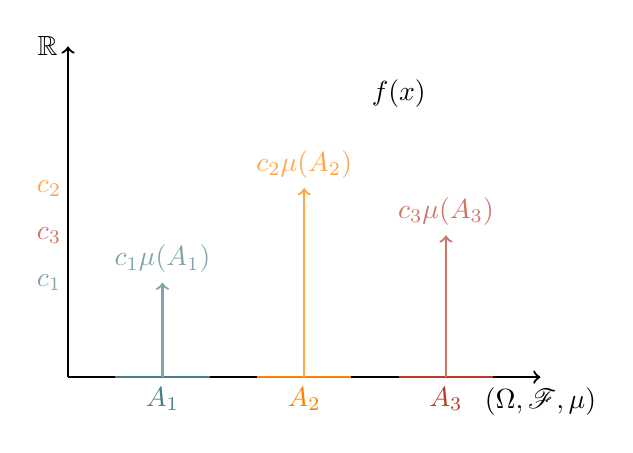
\begin{tikzpicture}[scale=1.2]

% Axes
\draw[thick, ->] (0,0) -- (5,0) node[below] {$(\Omega, \mathscr{F}, \mu)$}; % x-axis
\draw[thick, ->] (0,0) -- (0,3.5) node[left] {$\mathbb{R}$}; % y-axis

% Labels for A1, A2, A3 on x-axis
\draw[green, thick] (0.5,0) -- (1.5,0) node[midway, below] {$A_1$};
\draw[orange, thick] (2,0) -- (3,0) node[midway, below] {$A_2$};
\draw[red, thick] (3.5,0) -- (4.5,0) node[midway, below] {$A_3$};

% Bars representing c_i values
% Bar for A1
\draw[dashed, green!70] (1,0) -- (1,1) node[above, green!70] {$c_1 \mu(A_1)$};
\draw[->, thick, green!70] (1,0) -- (1,1);

% Bar for A2
\draw[dashed, orange!70] (2.5,0) -- (2.5,2) node[above, orange!70] {$c_2 \mu(A_2)$};
\draw[->, thick, orange!70] (2.5,0) -- (2.5,2);

% Bar for A3
\draw[dashed, red!70] (4,0) -- (4,1.5) node[above, red!70] {$c_3 \mu(A_3)$};
\draw[->, thick, red!70] (4,0) -- (4,1.5);

% Labels for c1, c2, c3 on the left
\node[green!70] at (-0.2,1) {$c_1$};
\node[orange!70] at (-0.2,2) {$c_2$};
\node[red!70] at (-0.2,1.5) {$c_3$};

% Function label
\node at (3.5,3) {$f(x)$};

\end{tikzpicture}
	
\end{eg}


\begin{df}{Lebesgue Integral (for Simple Functions)}\\
Define the set 
\[
S^+ := \{ f : \Omega \to \mathbb{R} \mid f\text{ is simple function, } f \geq 0 \}.
\]
For \( f \in S^+ \): define its Lebesgue integral w.r.t. its measure $\mu$ as: 
\[
\int_\Omega f \, d\mu := \sum_{i=1}^n c_i \cdot \mu(A_i), \quad \forall f \in S^+
\]
\end{df}
\textbf{Notation:} 
\[
\int_\Omega f \, d\mu \quad \text{or} \quad \int_\Omega f(x) \, d\mu(x).
\]

\begin{prop}{Lebesgue Integral}
\begin{itemize}
    \item \textbf{Linearity:} \( \int_\Omega (\alpha f + \beta g) \, d\mu = \alpha \int_\Omega f \, d\mu + \beta \int_\Omega g \, d\mu, \quad \forall f, g \in S^+, \alpha, \beta \geq 0. \)
    \item \textbf{Monotonicity:} If \( f \leq g \), then \( \int_\Omega f \, d\mu \leq \int_\Omega g \, d\mu. \)
\end{itemize}	
\end{prop}

\subsection{Lebesgue Integral}
\begin{df}{Lebesgue Integral}
\begin{enumerate}
	\item For any \( f: \Omega \to \mathbb{R} \), define the set $\mathcal{S_f}^+ = \qty{h\in S^+\mid h<f}$.
	\item Compute all Lebesgue integral $I(h)$ according to the previous definition. 
\end{enumerate}
We define 
$$\int_\Omega fd\mu = \sup_{h\in \mathcal{S_f}^+} I(h)$$
And we note that $f$ is $\mu$-integrable (or just integrable if the context if clear) if $\int_\Omega fd\mu <\infty$. 
\end{df}

\subsection{Important results and theorems}

\begin{lem}{Fatou's Lemma}
\noindent Given a measure space $(\Omega, \mathscr{F}, \mu)$ and a sequence of measurable, non-negative functions $\qty{f_n}$ each maps from $(\Omega, \mathscr{F}, \mu) \rightarrow (\R, \mathscr{B}, \cdot)$. Define a function $f \equiv \liminf_{n\to \infty} f_n(x)$, then $f$ is measurable and we have the following inequality: 
$$\int_\Omega f \, d\mu \leq \liminf_{n\to\infty} \int_\Omega f_n \, d\mu$$
\end{lem}

\begin{cor}{Beppo Levi's Monotone Convergence}
Let \((\Omega, \mathscr{F}, \mu)\) be a measure space, and let $\{X_n\}$ be a sequence of non-negative measurable functions defined on $\Omega$. Suppose:
$$0 \leq X_n(\omega) \leq X_{n+1}(\omega) \quad \forall \omega \in \Omega \quad \text{(monotonically increasing sequence of functions)}$$
Define the pointwise limit function:

$$X(\omega) = \lim_{n \to \infty} X_n(\omega), \quad \forall \omega \in \Omega$$
Then:
$$\lim_{n \to \infty} \int_\Omega X_n \, d\mu = \int_\Omega X \, d\mu$$
\end{cor}

\begin{thm}{Lebesgue's Dominated Convergence Theorem}
	\noindent Let $(\Omega, \mathscr{F}, \mu)$ be a measure space, and let $\{f_n\}$ be a sequence of measurable functions mapping from $(\Omega, \mathscr{F}, \mu)$ to $(\mathbb{R}, \mathscr{B})$. Suppose:  
\begin{itemize}
    \item \( f_n \to f \) pointwise almost everywhere on \( \Omega \), and  
    \item there exists an integrable function \( g \colon \Omega \to \mathbb{R} \) such that \( |f_n(\omega)| \leq g(\omega) \) for all \( \omega \in \Omega \) and all \( n \in \mathbb{N} \).
\end{itemize}
	
	Then all $f_n$ and $f$ integrable, and 
	$$\lim_{n\to\infty} \int_\Omega f_n d\mu = \int_\Omega \lim_{n\to\infty} f_n d\mu = \int_\Omega f d\mu$$
\end{thm}


\subsection{Expectation}

\begin{df}{Expectation}
Consider a measure space $(\Omega, \mathscr{F}, P)$ and a random variable $X: \Omega \rightarrow \R$. Its expectation is defined to be a Lebesgue integral
$$\E[X] = \int_\Omega X(\omega) dP(\omega)$$
\end{df}

\begin{cor}{Jensen's Inequality}
If  $X$  is a random variable and  $\phi: \R\rightarrow \R$  is a convex function, then:
$$\phi(\mathbb{E}[X]) \leq \mathbb{E}[\phi(X)]$$
Special Case: For $\phi(x) = |x|$, we obtain:
$$\abs{\mathbb{E}[X]} \leq \mathbb{E}\qty[\abs{X}]$$
Intuition: The expectation of a convex function applied to  X  is at least as large as applying the function to the expectation of  X . Convexity “pulls the curve upwards,” leading to this inequality.
\end{cor}

\begin{cor}{Markov's Inequality}
For a non-negative random variable $X$ and any $\alpha > 0$. 

$$P(|X| > \alpha) \leq \frac{\mathbb{E}[|X|]}{\alpha}$$
Intuition: The probability that $X$ exceeds some threshold $\alpha$ is bounded by the ratio of its expected value to  $\alpha$. It provides an upper bound on tail probabilities.
\end{cor}

\end{document}